\begin{frame}
  \frametitle{Visualisation in FEniCS}

   Three main options for visualisation

  \begin{itemize}

  \item
    Built-in VTK plotting
  \item
    matplotlib
  \item
    ParaView
  \end{itemize}

\end{frame}

\begin{frame}[fragile]
\frametitle{Built-in VTK plotting}

  Built-in plotting functionality for FEniCS

  \begin{itemize}

	\item Plot meshes, functions, mesh functions

	\item Not available on all FEniCS installations

	\item Limited 3D capabilities
  \end{itemize}
  \begin{python}
from fenics import *
parameters["plotting_backend"] = "vtk"

mesh = UnitCubeMesh(16, 16, 16)
plot(mesh)
interactive()
 \end{python}

  \begin{center}
    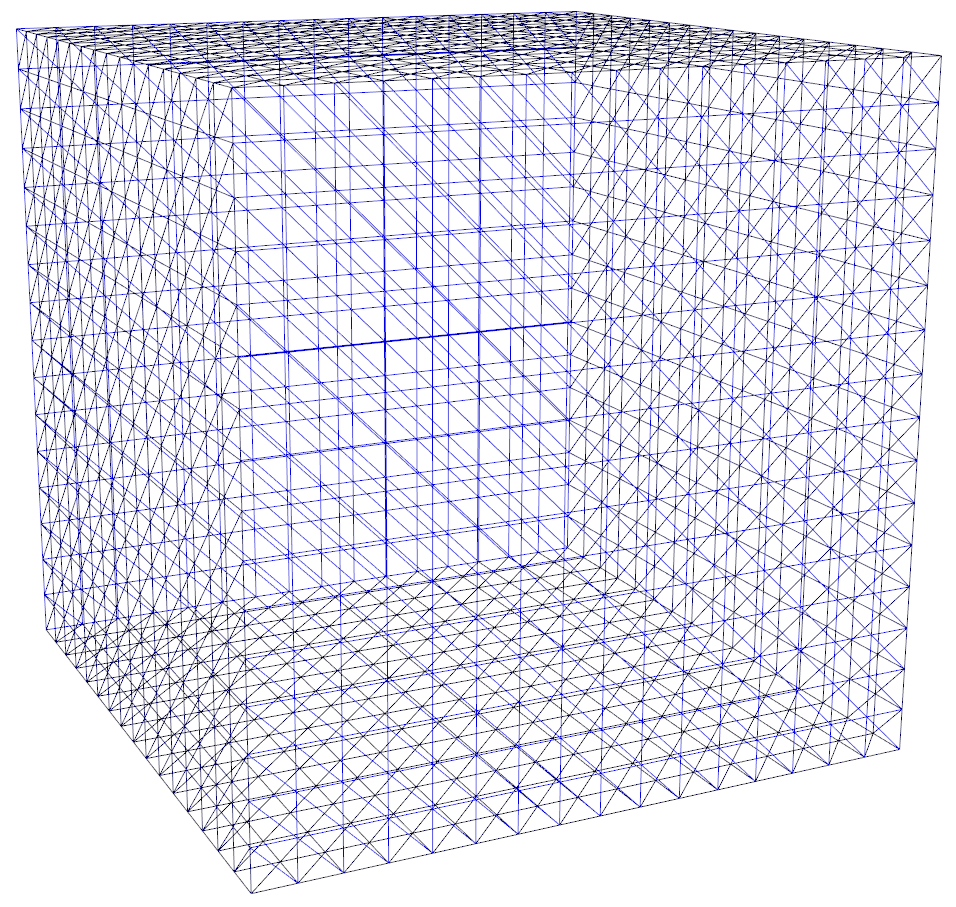
\includegraphics[width=3cm]{png/unitcube16.png}
  \end{center}


  \begin{python}

  \end{python}
\end{frame}

\begin{frame}[fragile]
\frametitle{matplotlib}

Plotting libarary for Python and Numpy

\begin{itemize}
  \item Part of a standard Python installation
  \item Has a MATLAB-like interface
  \item Produces high-quality 1D and 2D plots
\end{itemize}

Related projects
\begin{itemize}
   \item Pandas
   \item Seaborn
\end{itemize}

\end{frame}

\begin{frame}[fragile]
\frametitle{matplotlib example}

  \begin{python}
from dolfin import *
from matplotlib import pyplot
parameters["plotting_backend"] = "matplotlib"

mesh2D = UnitSquareMesh(16,16)
mesh3D = UnitCubeMesh(16, 16, 16)

plot(mesh2D)
plot(mesh3D)
pyplot.show()
  \end{python}
\end{frame}
\begin{frame}[fragile]
 \begin{minipage}{0.49\textwidth}
\begin{center}
    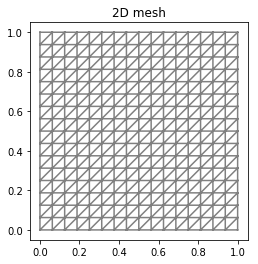
\includegraphics[width=\textwidth]{png/matplotlib_2D_mesh.png}
\end{center}
 \end{minipage}
 \begin{minipage}{0.49\textwidth}
\begin{center}
    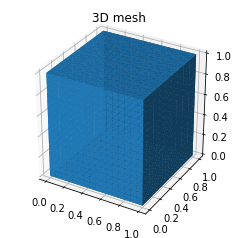
\includegraphics[width=\textwidth]{png/matplotlib_3D_mesh.png}
\end{center}
 \end{minipage}


\end{frame}


\begin{frame}[fragile]
\frametitle{matplotlib example II}
  \begin{python}
# appended to Cahn-Hilliard demo
parameters["plotting_backend"] = "matplotlib"
from matplotlib import pyplot

# call the plot command from dolfin
p = plot(u[0])

# set colormap
p.set_cmap("viridis")
p.set_clim(0.0, 1.0)

# add a title to the plot
pyplot.title("Cahn-Hilliard solution")

# add a colorbar
pyplot.colorbar(p);

# save image to disk
pyplot.savefig("demo_cahn-hilliard.png")
  \end{python}
\end{frame}
\begin{frame}[fragile]
\frametitle{matplotlib example II}
  \begin{center}
    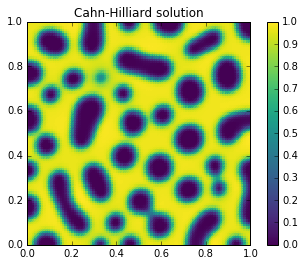
\includegraphics[width=8cm]{png/demo_cahn-hilliard.png}
  \end{center}

\end{frame}

\begin{frame}[fragile]
  \frametitle{matplotlib with FEniCS on mac and Windows}

  Displaying figures are more difficult when using a Docker installation of FEniCS

  The options are:
  \begin{enumerate}
    \item Saving figures to file and open them on the host system (inconvenient)
    \item Use Jupyter Notebook:

  Create and start a Docker container with the commands
    \begin{bash}
fenicsproject notebook fenics-nb stable
fenicsproject start fenics-nb
    \end{bash}
  Direct your web browser to address and port number printed to the screen

  \end{enumerate}
\end{frame}

\begin{frame}[fragile]
  \frametitle{Jupyter Notebook}

  Jupyter Notebook is part of the Project Jupyter ({\blue\url{www.jupyter.org}}), which evolved from IPython.
  \begin{itemize}
    \item Web application
    \item Provides interactive environment for Python code (and other languages!)
    \item Combine code, equations and visualisation in one interactive document

  \end{itemize}
To display figures inside the notebook, add this line to the notebook:
\begin{python}
  %matplotlib inline
\end{python}

\end{frame}
\begin{frame}[fragile]
\frametitle{ParaView}

  ParaView is a freely available, open source, multi-platform data visualisation application.
\begin{itemize}

  \item Publication-quality figures

  \item Provides sophisticated data analysis functions
    \begin{itemize}
      \item Stream lines
      \item Time averages
      \item Isosurfaces
      \item ... and much more
    \end{itemize}

  \item Can handle very large (and parallelized) data sets

  \item Support data file formats used by FEniCS:
    \begin{itemize}
      \item ParaView files (.pvd)
      \item VTK files (.vtu)
      \item XDMF files (.xdmf)
    \end{itemize}
\end{itemize}
\end{frame}

\begin{frame}[fragile]
\mbox{}



\begin{minipage}{0.59\textwidth}
\frametitle{ParaView resources}
  Official site: {\blue \url{www.paraview.org}}
  \begin{itemize}

    \item Binaries for mac, ubuntu, windows %(\url{www.paraview.org/dowload/}

    \item {\blue \hyperlink{http://www.paraview.org/tutorials/}{ParaView tutorials}}

    \item {\blue \hyperlink{http://www.paraview.org/paraview-guide/}{The ParaView Guide}}
  \end{itemize}
\end{minipage}
  \begin{minipage}{0.3\textwidth}
    \begin{center}
      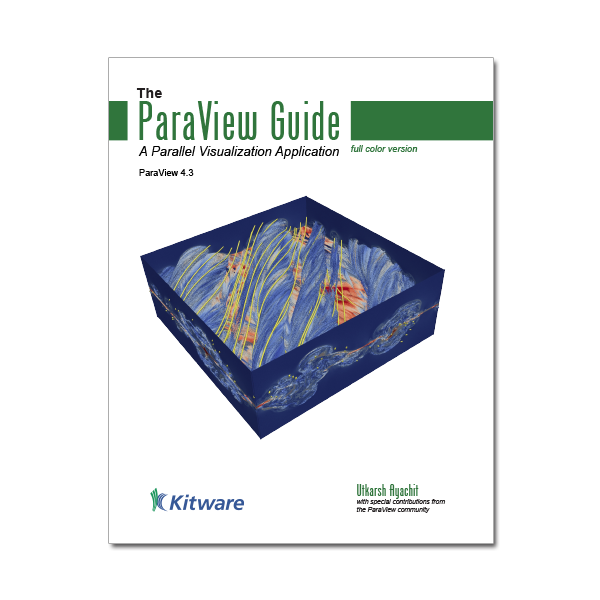
\includegraphics[width=\textwidth]{png/pv_book.png}
    \end{center}
  \end{minipage}



  \begin{minipage}{0.89\textwidth}
    \begin{center}
      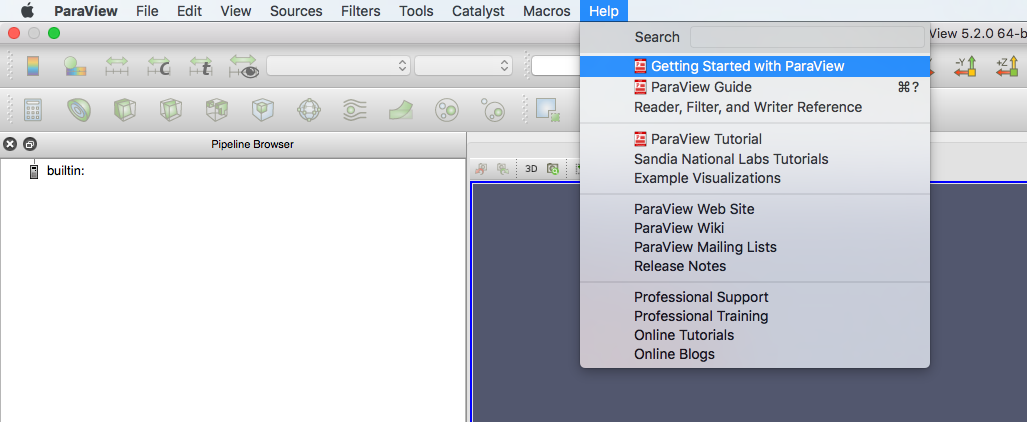
\includegraphics[width=\textwidth]{png/paraview_help_menu.png}
    \end{center}
  \end{minipage}
\end{frame}


\begin{frame}[fragile]
\frametitle{Using ParaView with FEniCS}
  Consider following example solving a Poisson problem:
  \begin{python}
from dolfin import *

mesh = UnitCubeMesh(16, 16, 16)
V = FunctionSpace(mesh, "P", 1)

u = TrialFunction(V)
v = TestFunction(V)
f = Constant(1.0)

a = inner(grad(u), grad(v)) * dx
L = f * v * dx

bc = DirichletBC(V, 0.0, "on_boundary")

uh = Function(V)
solve(a == L, uh, bc)
\end{python}

How can we visualise the solution?

\end{frame}

\begin{frame}[fragile]
\frametitle{Using ParaView with FEniCS}
First step is to store the solution to disk
  \begin{python}
# save solution in XDMF format
file = XDMFFile("output.xdmf")
file.write(uh, 0)
  \end{python}
\bigskip
  Alternatively save as .pvd format
  \begin{python}
# save solution in ParaView format
file = File("output.pvd")
file << uh
  \end{python}
\end{frame}

\begin{frame}[fragile]
\frametitle{Using ParaView with FEniCS}
  Start ParaView and open the file
  (Button in top left corner)
  \begin{center}
    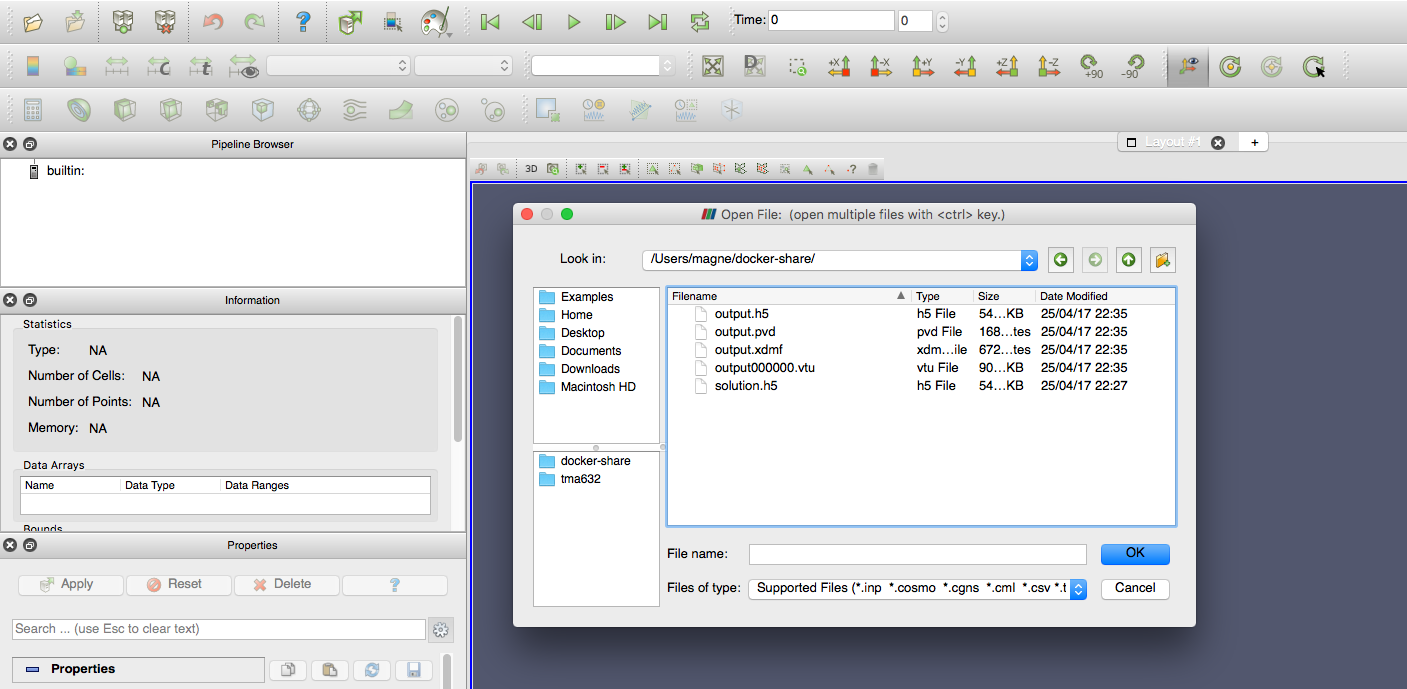
\includegraphics[width=\textwidth]{png/paraview_open.png}
  \end{center}
  After opening the file click the Apply button
\end{frame}

\begin{frame}[fragile]
\frametitle{Using ParaView with FEniCS}
  Your screen should look similar to this:
  \begin{center}
    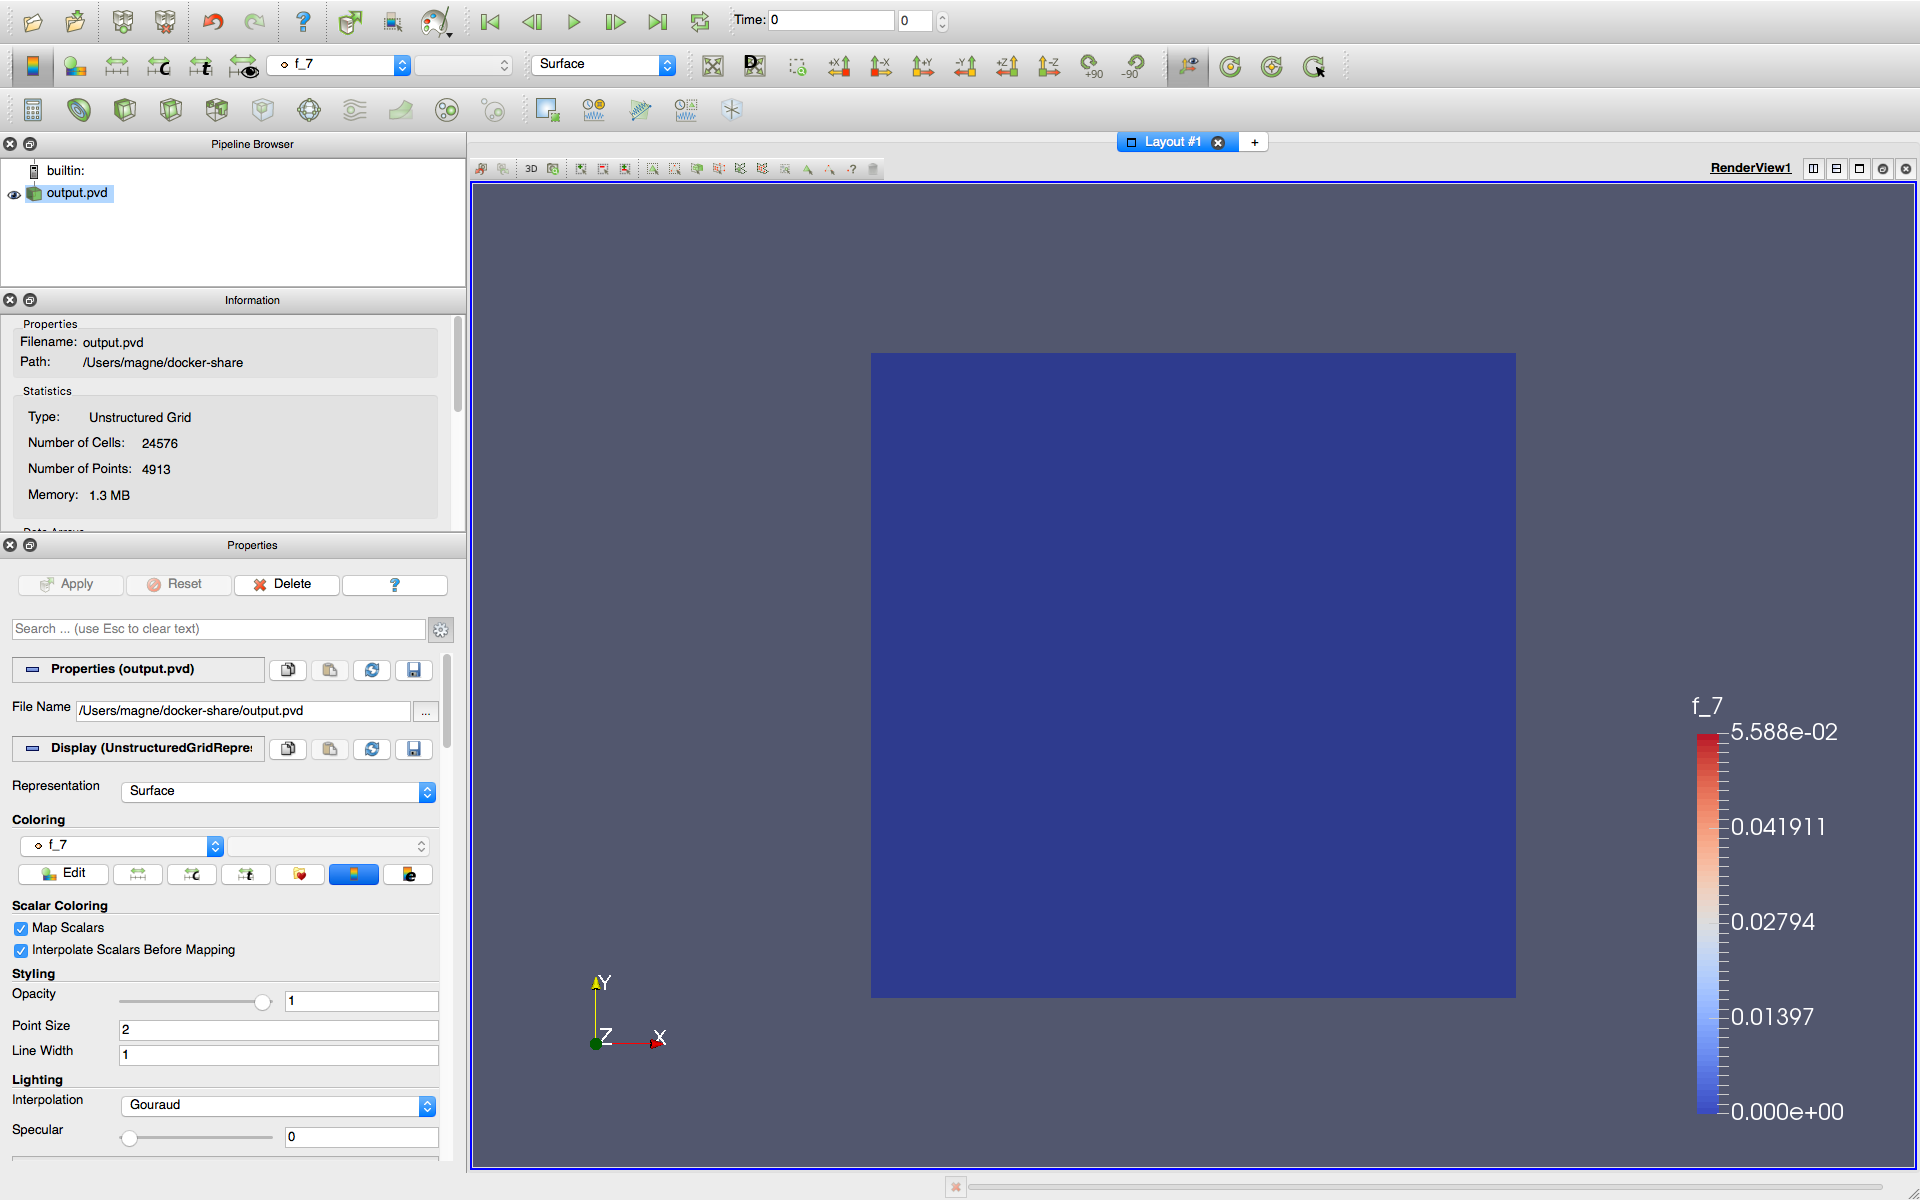
\includegraphics[width=\textwidth]{png/paraview_screen.png}
  \end{center}
  After opening the file click the Apply button
\end{frame}


\begin{frame}[fragile]
\frametitle{Using ParaView with FEniCS}
  ParaView has a nice GUI so you can easily play around with the many functions and settings available.

  \bigskip

  The functions for slicing, and contours and streamlines are particularly useful for 3D data:
  \begin{center}
    
\includegraphics[width=\textwidth]{png/paraview_buttons.png}
  \end{center}
  Save results using \pyth{File->Save Screenshot} or \pyth{File->Export Scene} from the menu.
\end{frame}

\begin{frame}[fragile]
\frametitle{Good practices for visualisation of data}

  \emph{Automate} visualisation (and other post-processing) with Python scripting.

  \begin{itemize}
  \item Ensures consistent results
  \item Saves time
  \item With ParaView: Manually make your figures \emph{once} using the GUI. You can save the state (\pyth{File->Save State}) and reuse it your python scripts.
  \end{itemize}

  \emph{Separate} post-processing from solver code.

\end{frame}
